\documentclass{templateNote}
\usepackage{tcolorbox}
\usepackage{hyperref}
\usepackage{amsmath}
\usepackage{amssymb}
\usepackage{array}
\usepackage{soul}
\usepackage{circuitikz}
\usepackage{float}
\usepackage[inline]{enumitem}
\usepackage{multicol}
\usepackage{colortbl}
\usepackage{tikz}
\usepackage{xcolor}
\usepackage[table]{xcolor}



\begin{document}
\imagenlogoU{img/logoNGMFormal_sinF.png}
\linklogoU{https://github.com/NicoGomezM} 
% \imagenlogoD{img/logo-ubb-txt-face.png} 
\titulo{Certamen 3}
\asignatura{Administración y programación de base de datos}
\autor{
    \indent
    Nicolás {Gómez Morgado}
}


\portada
\margenes 
% \tableofcontents
% \newpage


\section{Ejercicios guía 1}

\begin{enumerate}
    \item Supongamos que estamos utilizando un sistema de disco donde el tiempo para mover la cabeza de lectura/escritura a un bloque de 15ms, y el tiempo de transferencia de un bloque es de 0.4ms. Supongamos que queremos calcular el join de R con S, y tenemos que B(R)=1000, B(S)=500 y M=101. Para acelerar el join, queremos leer y escribir tantos bloques como podamos en posiciones consecutivas del disco, y usar buffers que puedan ser múltiplos de un bloque. Responda las siguientes preguntas. \\\\
    Tiempo en mover cabeza a un bloque: 15ms.\\
    Tiempo transferencia de un bloque: 0.4ms \\
    \underline{$R \Join S$}\\
    \hspace*{0.25cm} B(R) = 1000 \\
    \hspace*{0.25cm} B(S) = 500 \\
    \hspace*{0.25cm} M = 101 $\rightarrow$ 100 (Se deja uno para la salida)\\
    \begin{enumerate}[label=\alph*)]
        \item ¿Cuantas E/S de disco se requieren para realizar esta operación join? \\

        \begin{tabular}{|m{2cm}|m{6cm}|m{4cm}|}
            \hline
            $1^{er}$ pasada & Leer M bloques de R en MP[Memoria principal] (ordenar, escribir contenido ordenando) & 2B(R) crear sublistas ordenadas \\
            \hline
            $2^{da}$ pasada & El atributo de ordenación y unión & B(R) leer cada sublista \\
            \hline
            & Total & 3B(R) \\
            \hline
        \end{tabular}
        
        \vspace{0.5cm}
        \noindent Que para R son 3B(R), por lo tanto para S, es lo mismo 3B(S). \\Se rquiere B(R) + B(S). \\

        \textbf{Total: }\\
        Lo mismo para S $\rightarrow$ 3B(S) App. requerimientos [$\sqrt[]{{B(R)+B(S)}}$]\\
        \begin{align*}
            \textnormal{Disco E/S} &= 3(B(R)+B(S)) \\
            &= 3(1000+500) \\
            &= 4500 \\ 
        \end{align*}
        Por lo tanto son necesarias 4500 E/S de disco para realizar la union.\\

        \item ¿Cuanto tiempo toma un join basado en ordenamiento (sort-merge join), suponiendo que escribimos sublistas ordenadas en bloques consecutivos del disco? \\
        
        \textit{Datos:}\\
        SB(R) = Sublista de R = $\frac{B(R)}{M} = \frac{1000}{100}$ = 10 \\
        SB(S) = Sublista de S = $\frac{B(S)}{M} = \frac{500}{100}$ = 5 \\
        tt = Tiempo de transferencia = \textcolor{blue}{0.4ms.}\\
        M = 101 $\rightarrow$ 100 (Se deja uno para la salida)\\
        tm = Tiempo de mover la cabeza = 15ms.\\

        \begin{tabular}{|m{2cm}|m{12cm}|}
            \hline
            $1^{er}$ pasada & R (Lectura y escritura) y S (Lectura y escritura): misma pista de lectura/escritura secuenciales \\
            \hline
            & tm + (SB(R) $\cdot$ 2((M-1)$\cdot$tt) +tm + (SB(S) $\cdot$ 2((M-1)$\cdot$tt)) + S(B(S)) \\
            & $[15+(10)\cdot[2\cdot(100\cdot\textcolor{blue}{0.4})]]+[15+(5\cdot[2\cdot(100\cdot\textcolor{blue}{0.4})])]$ \\ 
            & $[15+(10)\cdot[80]]+[15+(5\cdot[80])]$ \\
            & $[15+800]+[15+400]$ \\
            & $815+415$ \\
            & 1230 ms. \\
            \hline
        \end{tabular}

        \begin{tabular}{|m{2cm}|m{6cm}|m{6cm}|}
            \hline
            $2^{da}$ pasada & Original \newline 15 buffers c/u con 1 bloque & Nueva: 15 buffers c/u con 6 bloques\\
            \hline
            & M/bloques $\cdot$ buffers $\cdot$ tm & M/bloques $\cdot$ buffers $\cdot$ tm \\
            & = 100 times $\cdot$ 15 buffers $\cdot$ 15 ms & 17 times $\cdot$ 15 buffers $\cdot$ 15 ms \\
            & = 25500 ms = 22.5 seg & $\backsim$ 3825 ms $\backsim$ 3.825 seg\\
            \hline
        \end{tabular}
        
        \begin{align*}
            1 \textnormal{ buffer} + 1 \textnormal{ bloque} &= 1230 ms + 22500 ms = 23730 ms \approx 23.7 seg.\\ %TODO:Destacar de azul
            1 \textnormal{ buffer} + 6 \textnormal{ bloques} &= 1230 ms + 3825 ms = 5055 ms \approx 5.05 seg.\\ %TODO:Destacar de rojo
        \end{align*}
    \end{enumerate}

    \item Supongamos que tenemos las relaciones $R(a,b)$ , $S(b,c)$ , $T(c,d)$ , $U(d,e)$ con las siguientes características:
        
        \begin{center}
            \begin{minipage}{0.3\textwidth}
                T(R) = 100 \\
                V(R,b) = 100 \\
                T(S) = 100 \\
                V(S,b) = 100 \\
                V(S,c) = 10 \\
                \end{minipage}%
                \begin{minipage}{0.3\textwidth}
                T(T) = 100 \\
                V(T,c) = 10 \\
                V(T,d) = 100 \\
                T(U) = 100 \\
                V(U,d) = 100 \\
            \end{minipage}
        \end{center}    

        \noindent Computar un orden de Join de R sobre S Sobre T Sobre U [$R \Join S \Join T \Join U$], utilizando:

        \begin{enumerate}[label=\alph*)]
            \item Dinámica (Dynamic Programming method) \\
            
                \begin{center}
                    \begin{tabular}{|c|c|c|c|}
                        \hline
                        R & S & T & U \\
                        \hline
                        100 & 100 & 100 & 100 \\
                        \hline
                        0 & 0 & 0 & 0 \\
                        \hline
                        R & S & T & U \\
                        \hline
                    \end{tabular}
                \end{center}

                Considerando los pares: \\

                1) $R \Join S = 100$ \\
                2) $R \Join T = 10000$ \\
                3) $R \Join U = 10000$ \\
                4) $S \Join T = 1000$ \\
                5) $S \Join U = 10000$ \\
                6) $T \Join U = 100$ \\

                \begin{center}
                    \begin{tabular}{|c|c|c|c|c|c|c|}
                        \hline
                        & R,S & R,T & R,U & S,T & S,U & T,U\\
                        \hline
                        Size & 100 & 10000 & 10000 & 1000 & 10000 & 100 \\
                        \hline
                        Cost. & & & & & &  \\
                        \hline
                        Best plan & & & & & &  \\
                        \hline
                    \end{tabular}
                \end{center}
                
                \noindent Ahora considerar la unión de 3 de las 4 relaciones. Elegir 2 para unir primero.\\
                \begin{center}
                    {R,S,T}{R,S,U}{R,T,U}{S,T,U}
                \end{center}

                1) (R,S,T) = \\
                \hspace*{0.25cm}$R \Join S = 100  \leftarrow$ \\
                \hspace*{0.25cm}$R \Join T = 10000$ \\
                \hspace*{0.25cm}$S \Join T = 1000$ 
                \begin{align*}
                    T((R \Join S) \Join T) &= \frac{T(R \Join S)\cdot T(T)}{\max\{V(R \Join S,c),V(T,c)\}} = \frac{100\cdot100}{max\{10,10\}} \\ 
                    &= \frac{10000}{10} = 1000 
                \end{align*}
                
                2) (R,S,U) = \\
                \hspace*{0.25cm}$R \Join S = 100 \leftarrow$ \\
                \hspace*{0.25cm}$R \Join U = 10000$ \\
                \hspace*{0.25cm}$S \Join U = 10000$ \\

                \begin{align*}
                    T((R \Join S) \Join U) &= \frac{T(R \Join S)\cdot T(U)}{\max\{V(R \Join S,c),V(U,c)\}} = \frac{1000\cdot100}{max\{10,10\}} \\ 
                    &= \frac{100000}{10} = 10000
                \end{align*}
                
                3) (R,T,U) = \\
                \hspace*{0.25cm}$R \Join T = 10000$ \\
                \hspace*{0.25cm}$R \Join U = 10000$ \\
                \hspace*{0.25cm}$T \Join U = 100 \leftarrow$

                \begin{align*}
                    T((R \Join T) \Join U) &= \frac{T(R \Join T)\cdot T(U)}{\max\{V(R \Join T,d),V(U,d)\}} = \frac{10000\cdot100}{max\{100,100\}} \\ 
                    &= \frac{1000000}{100} = 10000
                \end{align*}

                4) (S,T,U) = \\
                \hspace*{0.25cm}$S \Join T = 1000$ \\
                \hspace*{0.25cm}$S \Join U = 10000$ \\
                \hspace*{0.25cm}$T \Join U = 100 \leftarrow$

                \begin{align*}
                    T((S \Join T) \Join U) &= \frac{T(S \Join T)\cdot T(U)}{\max\{V(S \Join T,d),V(U,d)\}} = \frac{1000\cdot100}{max\{100,100\}} \\ 
                    &= \frac{100000}{100} = 1000
                \end{align*}

                \begin{tabular}{|c|c|c|c|c|}
                    \hline
                    & RST & RSU & RTU & STU \\
                    \hline
                    S & 1000 & 10000 & 10000 & 1000 \\
                    \hline
                    C & 100 & 100 & 100 & 100  \\
                    \hline
                    P & $(R \Join S) \Join T$ & $(R \Join S) \Join U$ & $(T \Join U) \Join R$ & $(T \Join U) \Join S$ \\
                    \hline
                \end{tabular}
                
                \noindent Tripletes. \\Considerar arboles. \\

                \begin{figure}[H]
                    \centering
                    
\includegraphics[width=\textwidth]{img/img1.png}
                \end{figure}
                
                \noindent \textbf{Agrupando:} \\
                \textbf{Costo mas tamaño de cada triplet} \\
                \begin{math}
                    (((R \Join S ) \Join T ) \Join U) = 1000 + 100 = \tikz[baseline=(char.base)]{\node[shape=circle,draw,inner sep=2pt] (char) {$1100$};} \\
                    (((R \Join S ) \Join U ) \Join T) = 10000 + 100 = 10100 \\
                    (((R \Join T ) \Join U ) \Join S) = 10000 + 100 = 10100 \\
                    (((S \Join T ) \Join U ) \Join R) = 1000 + 100 = \tikz[baseline=(char.base)]{\node[shape=circle,draw,inner sep=2pt] (char) {$1100$};} \\
                \end{math}

                \begin{figure}[H]
                    \centering
                    
\includegraphics[width=\textwidth]{img/img2.png}
                \end{figure}

                \noindent \textbf{Agrupando:} \\
                \begin{math}
                    (T \Join U) \Join (R \Join S) = 100 + 100 = 200 \leftarrow\\
                    (S \Join U) \Join (R \Join U) = 10000 + 1000 = 11000 \\
                    (R \Join T) \Join (S \Join U) = 10000 + 10000 = 20000 \\
                \end{math}

            
            \item Greedy method\\
            \noindent \textbf{Se toma una decision sin retroceder.} \\
            \noindent \underline{Base:} Pares de relaciones cuyo tamaño estimado es el mas pequeño (árbol actual).

            \noindent % Evita la indentación en la primera línea
            \begin{center}
            \begin{minipage}{0.3\textwidth}
            \begin{align}
                {R,S} &= 100 \\
                {R,T} &= 10000 \nonumber \\
                {R,U} &= 10000 \nonumber 
            \end{align}
            \end{minipage}%
            \begin{minipage}{0.3\textwidth}
            \begin{align}
                {S,T} &= 10000 \nonumber \\
                {S,U} &= 10000 \nonumber \\  
                {T,U} &= 100 
            \end{align}
            \end{minipage}   
            \end{center}

            \vspace{0.5cm}
            \noindent Inducción: Encontrar todas las relaciones no incluidas, en este caso, T y U.

            \begin{align*}
                R \Join S &- ((R \Join S) \Join U) = 10000 \\
                R \Join S &- ((R \Join S) \Join T) = 1000 \\
            \end{align*}
            
            Se escoge T. Luego hay que unirse a U, no hay mas opciones.
            \begin{align*}
                (((R \Join S)\Join T)\Join U) = 1100
            \end{align*}

            \begin{figure}[H]
                \centering
                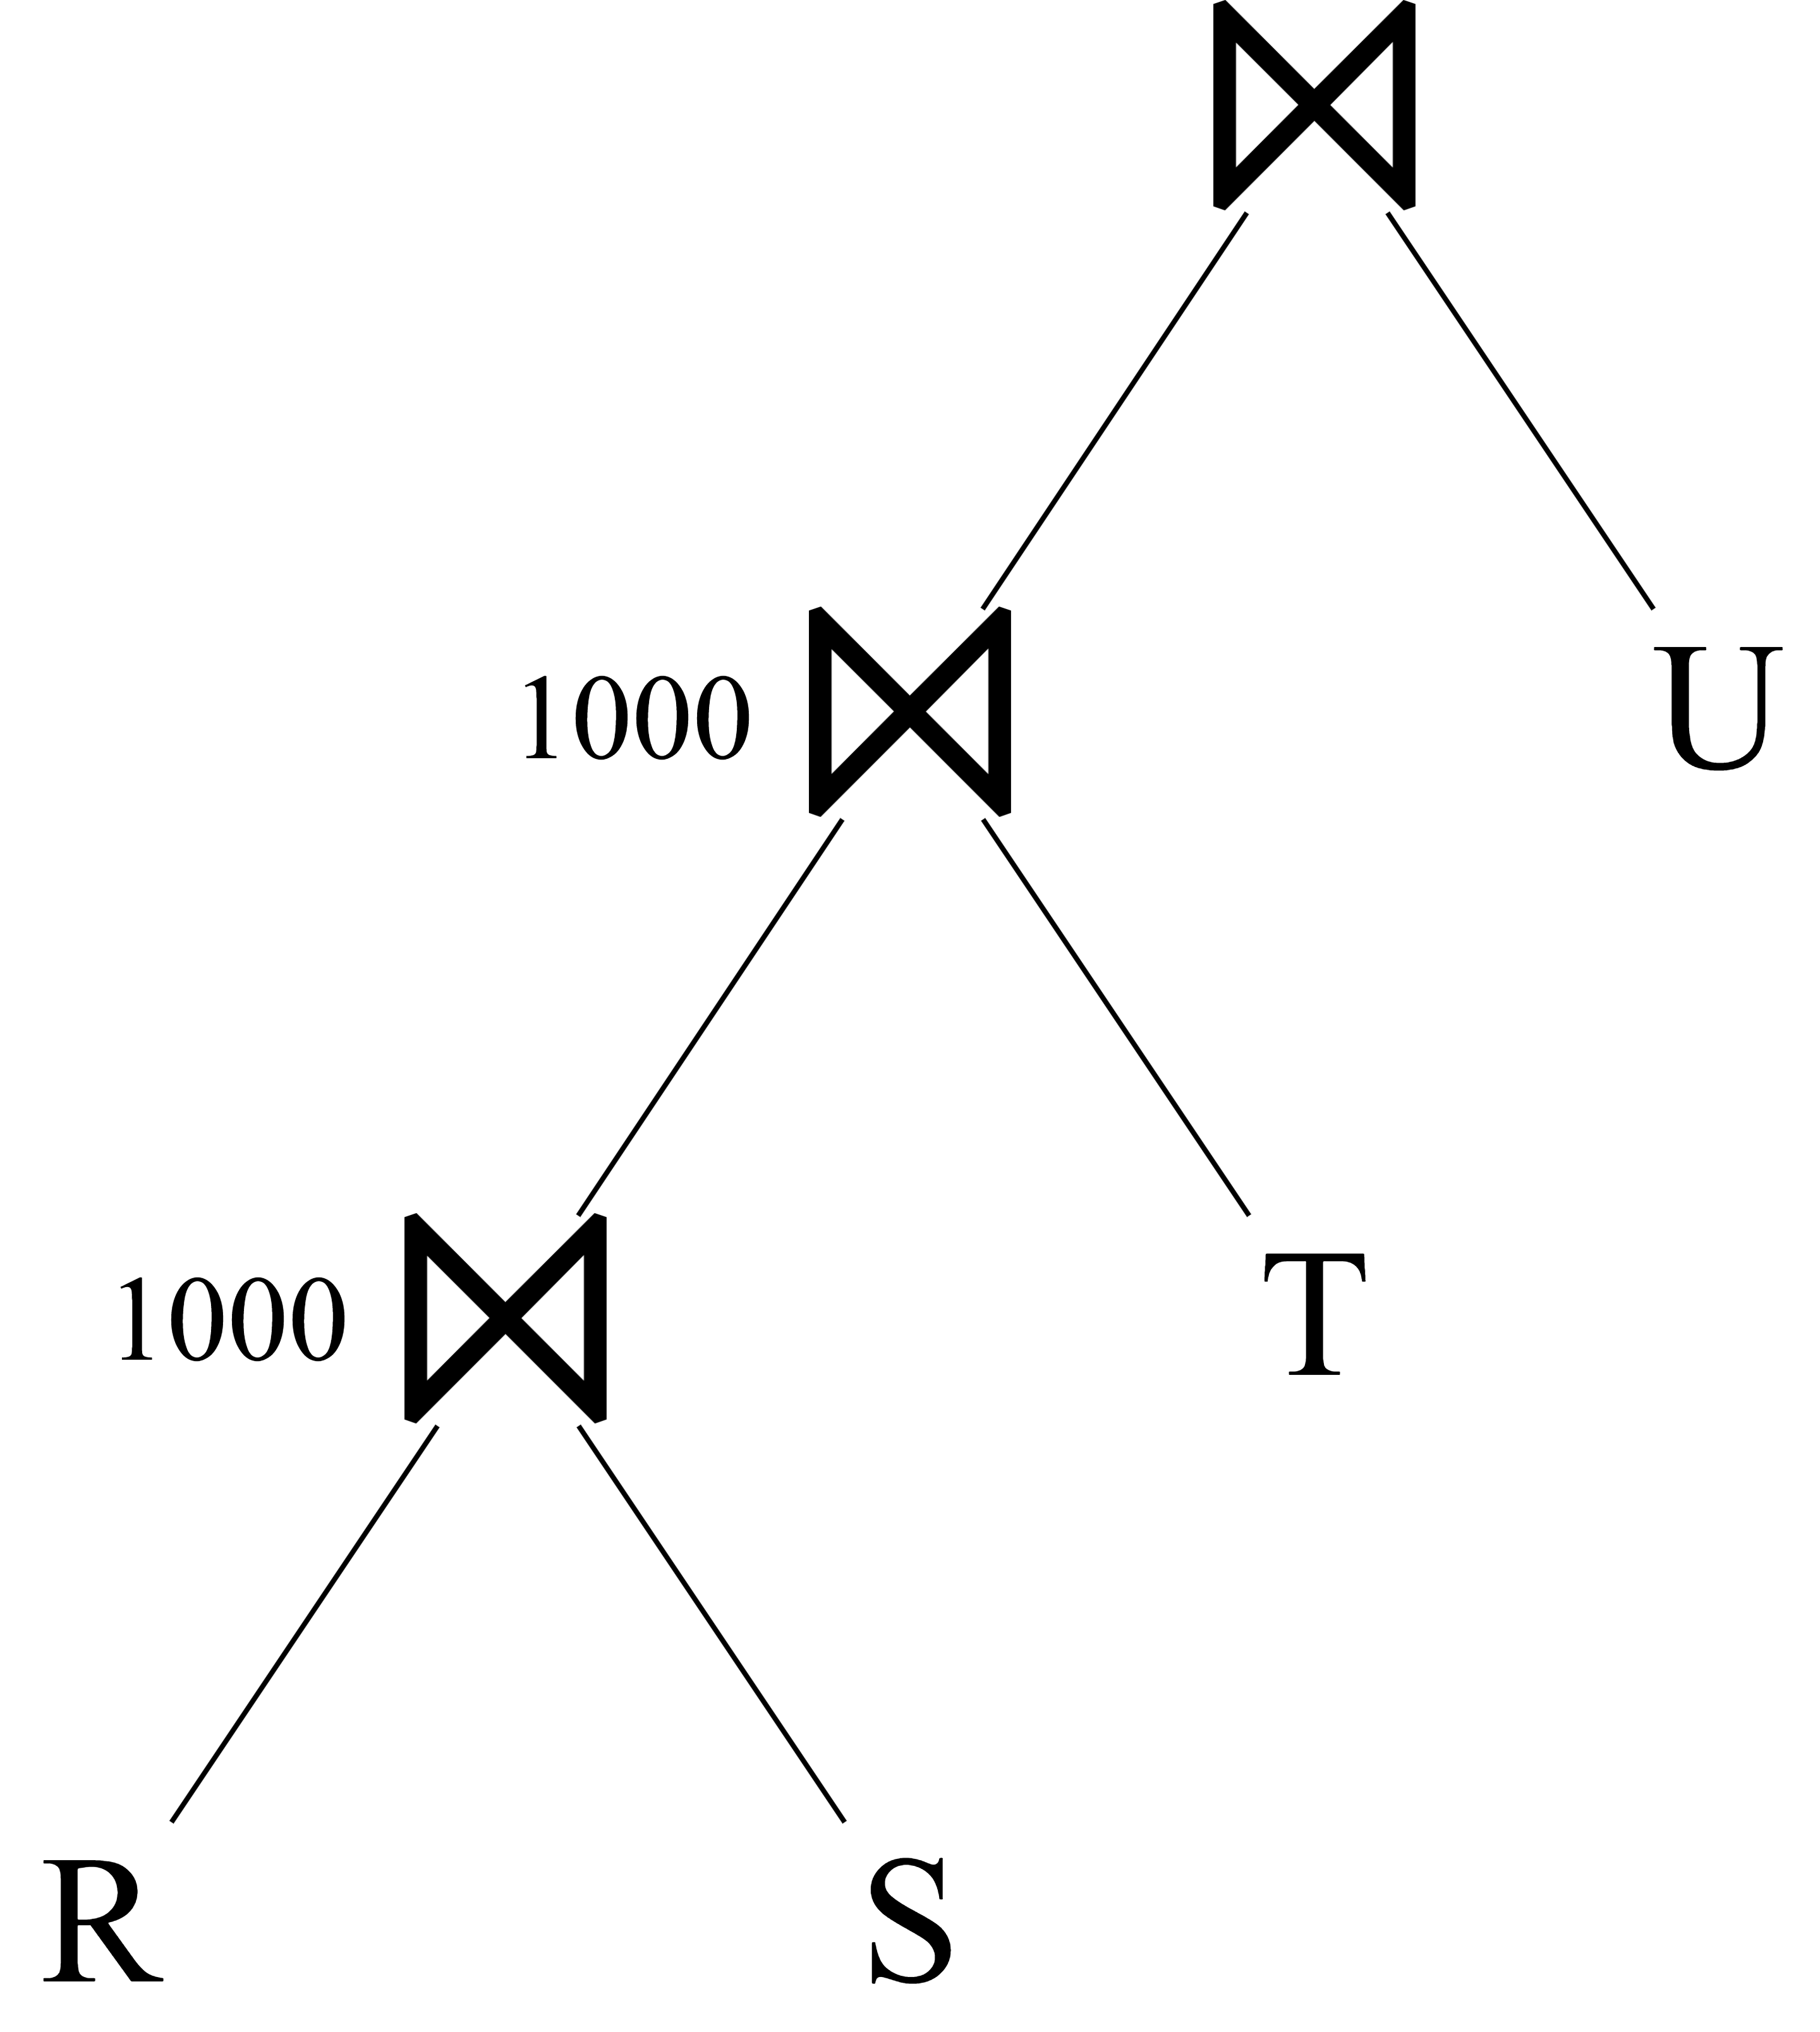
\includegraphics[width=5cm]{img/img3.png}
            \end{figure}

        \end{enumerate}

\end{enumerate}

\newpage
\section{Ejercicios guía 2}
\begin{enumerate}
    \item Traspasar la consulta SQL a un árbol de consulta.     
\end{enumerate}

\begin{itemize}
    \item SELECT apellido1
    \item FROM Empleado E, trabajaEn T, proyecto P
    \item WHERE nameProy=’aquarius’
    \item AND T.idProy = P.idProy
    \item AND E.idEmpleado = T.idEmpleado
    \item AND E.FechaNacimiento>'1957-12-21'
    \begin{itemize}
        \item Obtener el árbol inicial (canónico) de la consulta

        \begin{center}
            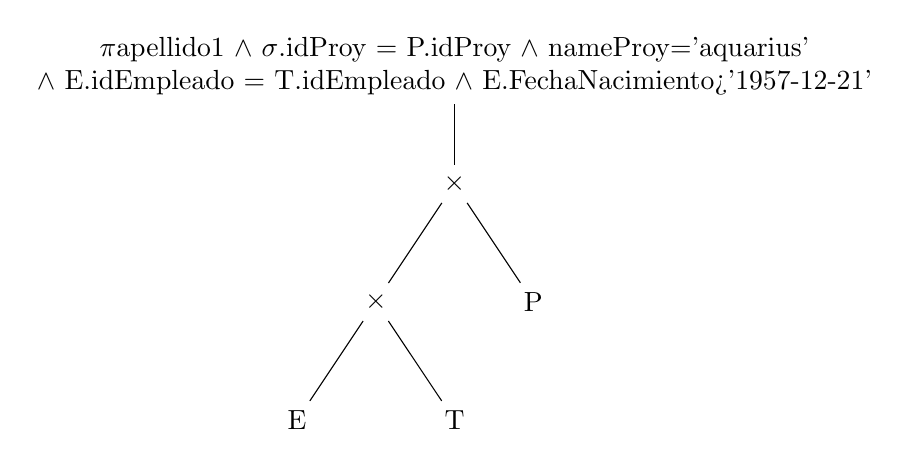
\begin{tikzpicture}[level distance=1.5cm,
                level 1/.style={sibling distance=3.5cm},
                level 2/.style={sibling distance=2cm}]
                \node[align=center] {$\pi$apellido1 $\land$ $\sigma$.idProy = P.idProy $\land$ nameProy='aquarius' \\ $\land$ E.idEmpleado = T.idEmpleado $\land$ E.FechaNacimiento>'1957-12-21'}
                    child {node {$\times$}
                        child{node {$\times$}
                            child{node{E}}
                            child{node{T}}
                        }
                        child{node {P}}
                    };
            \end{tikzpicture}
        \end{center}

        \item Explique como se optimiza el árbol de consulta mediante la optimización vista en clases
    
        \begin{enumerate}[label=\alph*)]
            \item Separar selección y proyección por tablas.
            \begin{center}
                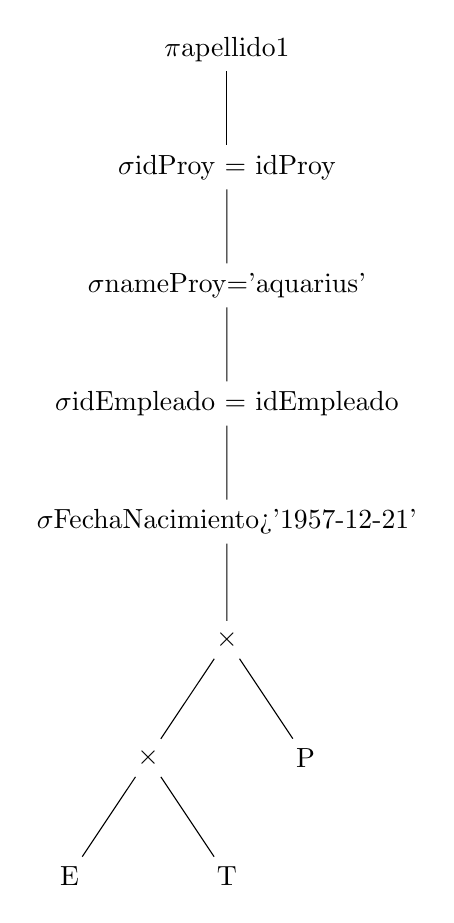
\begin{tikzpicture}[level distance=1.5cm,
                    level 1/.style={sibling distance=3.5cm},
                    level 2/.style={sibling distance=2cm}]
                    \node[align=center] {$\pi$apellido1}
                    child {node {$\sigma$idProy = idProy}
                        child {node {$\sigma$nameProy='aquarius'}
                            child {node {$\sigma$idEmpleado = idEmpleado}
                                child {node {$\sigma$FechaNacimiento>'1957-12-21'}
                                    child {node {$\times$}
                                        child{node {$\times$}
                                            child{node{E}}
                                            child{node{T}}
                                        }
                                        child{node {P}}
                                    }
                                }
                            }
                        }
                    };
                \end{tikzpicture}
            \end{center}
            \item Reorganizar las tablas buscando la forma mas optima de unir las tablas.
            \begin{center}
                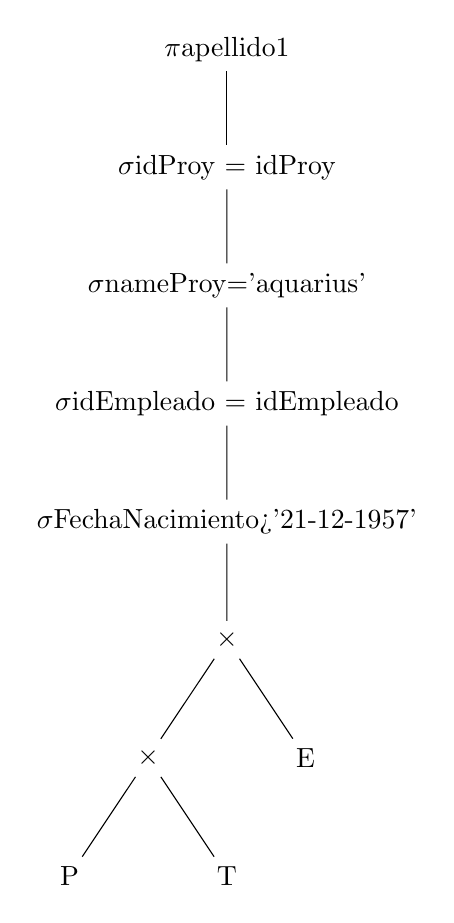
\begin{tikzpicture}[level distance=1.5cm,
                    level 1/.style={sibling distance=3.5cm},
                    level 2/.style={sibling distance=2cm}]
                    \node[align=center] {$\pi$apellido1}
                    child {node {$\sigma$idProy = idProy}
                        child {node {$\sigma$nameProy='aquarius'}
                            child {node {$\sigma$idEmpleado = idEmpleado}
                                child {node {$\sigma$FechaNacimiento>'21-12-1957'}
                                    child {node {$\times$}
                                        child{node {$\times$}
                                            child{node{P}}
                                            child{node{T}}
                                        }
                                        child{node {E}}
                                    }
                                }
                            }
                        }
                    };
                \end{tikzpicture}
            \end{center}
            \item Se bajan las selecciones hasta su producto cartesiano.
            \begin{center}
                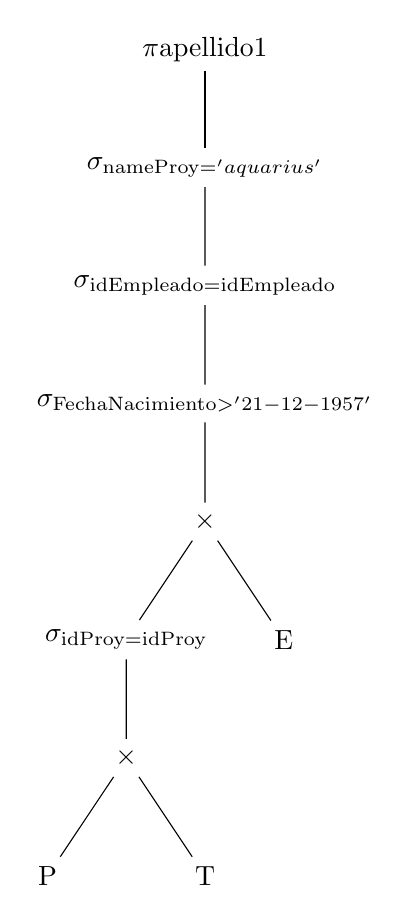
\begin{tikzpicture}[level distance=1.5cm,
                    level 1/.style={sibling distance=3.5cm},
                    level 2/.style={sibling distance=2cm}]
                    \node[align=center] {$\pi$apellido1}
                        child {node {$\sigma_{\text{nameProy}='aquarius'}$}
                            child {node {$\sigma_{\text{idEmpleado} = \text{idEmpleado}}$}
                                child {node {$\sigma_{\text{FechaNacimiento} > '21-12-1957'}$}
                                    child {node {$\times$}
                                        child{node{$\sigma_{\text{idProy} = \text{idProy}}$}
                                            child{node{$\times$}
                                                child{node{P}}
                                                child{node{T}}
                                            }
                                        }
                                        child{node {E}}
                                    }
                                }
                            }
                        }
                    ;
                \end{tikzpicture}
            \end{center} 
            
            \item Cambia la selección y producto cartesiano por un join.
            \begin{center}
                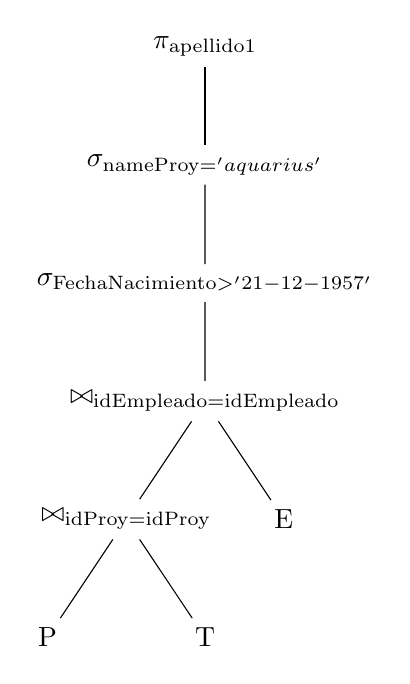
\begin{tikzpicture}[level distance=1.5cm,
                    level 1/.style={sibling distance=3.5cm},
                    level 2/.style={sibling distance=2cm}]
                    \node[align=center] {$\pi_{\text{apellido1}}$}
                        child {node {$\sigma_{\text{nameProy}='aquarius'}$}
                            child {node {$\sigma_{\text{FechaNacimiento} > '21-12-1957'}$}
                                child {node {$\bowtie_{\text{idEmpleado} = \text{idEmpleado}}$}
                                    child {node {$\bowtie_{\text{idProy} = \text{idProy}}$}
                                        child {node {P}}
                                        child {node {T}}
                                    }
                                    child {node {E}}
                                }
                            }
                        }
                    ;
                \end{tikzpicture}
            \end{center}

            \item Se bajan las selecciones a sus respectivas tablas.
            \begin{center}
                \begin{tikzpicture}[level distance=1.5cm,
                    level 1/.style={sibling distance=3.5cm},
                    level 2/.style={sibling distance=5cm}]
                    \node[align=center] {$\pi_{\text{apellido1}}$}
                        child {node {$\bowtie_{\text{idEmpleado} = \text{idEmpleado}}$}
                            child {node {$\bowtie_{\text{idProy} = \text{idProy}}$}
                                child {node {$\sigma_{\text{nameProy}='aquarius'}$}
                                    child {node {P}}
                                }
                                child {node {T}}
                            }
                            child {node {$\sigma_{\text{FechaNacimiento} > '21-12-1957'}$}
                                child {node {E}}
                            }
                        }
                    ;
                \end{tikzpicture}
            \end{center}

            \item Se proyecta solo lo necesario en subtotablas.
            \begin{center}
                \begin{tikzpicture}[level distance=1.5cm,
                    level 1/.style={sibling distance=3.5cm},
                    level 2/.style={sibling distance=5cm}]
                    \node[align=center] {$\pi_{\text{apellido1}}$}
                        child {node {$\bowtie_{\text{idEmpleado} = \text{idEmpleado}}$}
                            child {node {$\pi_{\text{idEmpleado}}$}
                                child {node {$\bowtie_{\text{idProy} = \text{idProy}}$}
                                    child {node {$\pi_{\text{idProy}}$}
                                        child {node {$\sigma_{\text{nameProy}='aquarius'}$}
                                            child {node {P}}
                                        }
                                    }
                                    child {node {$\pi_{\text{idProy, idEmpleado}}$}
                                        child {node {T}}
                                    }
                                }
                            }
                            child {node {$\pi_{\text{idEmpleado, apellido1}}$}
                                child {node {$\sigma_{\text{FechaNacimiento} > '21-12-1957'}$}
                                    child {node {E}}
                                }
                            }
                        }
                    ;
                \end{tikzpicture}
            \end{center}

        \end{enumerate}
    \end{itemize}
\end{itemize}

\begin{enumerate}
    \setcounter{enumi}{1}
    \newpage
    \item Considere las siguientes relaciones: \\
    \hspace*{0.25cm} Variedades(IdVar, Nombre, Prog2, Prog1) \\
    \hspace*{0.25cm} Predios(IdPredio, NombrePredio, Comuna, Superficie) \\
    \hspace*{0.25cm} Siembra(IdPredio, IdVar, HaSem, Rdto, añoA) 
    
    Sea la siguiente consulta: “Listar los nombres de las variedades sembradas en el predio idPredio = 10 y que el año 2015 tuvieron un rendimiento mayor a 60 qq/ha”.

    \begin{enumerate}[label=\alph*)]
        \item Escriba la consulta en SQL para la consulta anterior
        \begin{itemize}
            \item \textbf{SELECT} V.NOMBRE 
            \item \textbf{FROM} VARIEDADES V, SIEMBRA S
            \item \textbf{WHERE} S.IDPREDIO = 10 \\AND S.AÑOA = 2015 \\AND S.RDTO > 60 \\AND S.IDVAR = V.IDVAR
        \end{itemize}
        \item Escriba la consulta en A.Relacional para la consulta anterior
        \begin{equation*}
            \pi_{v.nombre} \Bigg( \sigma_{\substack{
                S.IdPredio = 10 \land \\
                \ S.añoA = 2015 \land \\
                \ S.Rdto > 60      
            }} \big( \text{VARIEDAD}\bowtie \text{SIEMBRA}) )
        \end{equation*}
        \item Obtener el árbol inicial (canónico) de la consulta
        \begin{center}
            \begin{tikzpicture}[level distance=1.5cm,
                level 1/.style={sibling distance=3.5cm},
                level 2/.style={sibling distance=5cm}]
                \node[align=center] {$\pi_{\text{nombre}} \land \sigma_{\substack{
                        \text{idVar} = \text{idVar} \land
                        \text{idPredio} = 10 \land
                        \text{añoA} = 2015 \land
                        \text{Rdto} > 60}}$}
                        child{node {$\times$}
                            child{node {V}}
                            child{node {S}}
                        }
                ;
            \end{tikzpicture}
        \end{center}
        \item Explique como se optimiza el árbol de consulta mediante el algoritmo de optimización algebraica (visto en clases)
        \begin{enumerate}
            \item Separar selección y proyección por tablas.
            \begin{center}
                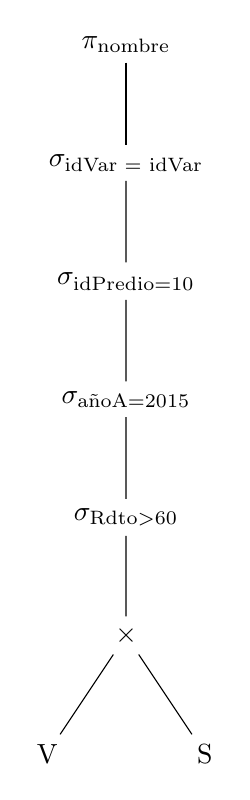
\begin{tikzpicture}[level distance=1.5cm,
                    level 1/.style={sibling distance=3.5cm},
                    level 2/.style={sibling distance=2cm}]
                    \node[align=center] {$\pi_{\text{nombre}}$}
                        child {node {$\sigma_{\textnormal{idVar = idVar}}$}
                            child {node {$\sigma_{\substack{\text{idPredio} = 10}}$}
                                child {node {$\sigma_{\text{añoA} = 2015}$}
                                    child {node {$\sigma_{\text{Rdto} > 60}$}
                                        child {node {$\times$}
                                            child {node {V}}
                                            child {node {S}}
                                        }
                                    }
                                }
                            }
                        };
                \end{tikzpicture}
            \end{center}
            \item Reorganizar las tablas buscando la forma mas optima de unir las tablas.
            Como solo son 2 tablas no es necesario reorganizar.
            \item Se bajan las selecciones hasta su producto cartesiano.
            \begin{center}
                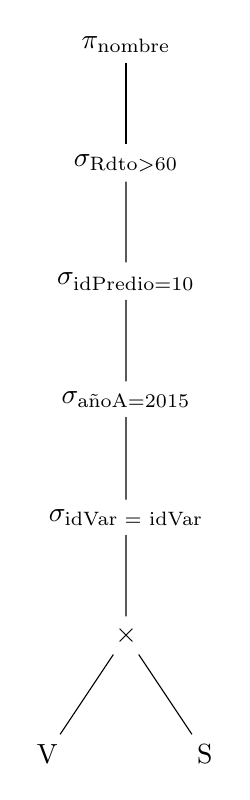
\begin{tikzpicture}[level distance=1.5cm,
                    level 1/.style={sibling distance=3.5cm},
                    level 2/.style={sibling distance=2cm}]
                    \node[align=center] {$\pi_{\text{nombre}}$}
                        child {node {$\sigma_{\text{Rdto} > 60}$}
                            child {node {$\sigma_{\substack{\text{idPredio} = 10}}$}
                                child {node {$\sigma_{\text{añoA} = 2015}$}
                                    child {node {$\sigma_{\textnormal{idVar = idVar}}$}
                                        child {node {$\times$}
                                            child {node {V}}
                                            child {node {S}}
                                        }
                                    }
                                }
                            }
                        };
                \end{tikzpicture}
            \end{center}

            \item Se cambian las selecciones y producto cartesiano por un join.

            \begin{center}
                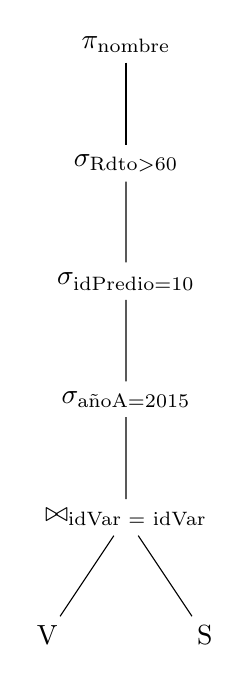
\begin{tikzpicture}[level distance=1.5cm,
                    level 1/.style={sibling distance=3.5cm},
                    level 2/.style={sibling distance=2cm}]
                    \node[align=center] {$\pi_{\text{nombre}}$}
                        child {node {$\sigma_{\text{Rdto} > 60}$}
                            child {node {$\sigma_{\substack{\text{idPredio} = 10}}$}
                                child {node {$\sigma_{\text{añoA} = 2015}$}
                                    child {node {$\bowtie_{\textnormal{idVar = idVar}}$}
                                        child {node {V}}
                                        child {node {S}}
                                    }
                                }
                            }
                        };
                \end{tikzpicture}
            \end{center}

            \item Se baja la selección a su respectiva tabla.
            \begin{center}
                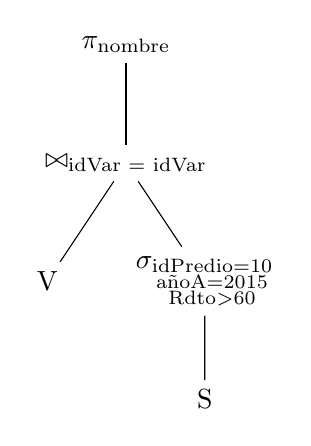
\begin{tikzpicture}[level distance=1.5cm,
                    level 1/.style={sibling distance=3.5cm},
                    level 2/.style={sibling distance=2cm}]
                    \node[align=center] {$\pi_{\text{nombre}}$}
                        child {node {$\bowtie_{\textnormal{idVar = idVar}}$}
                            child {node {V}}
                            child {node[align=center] {$\sigma_{\substack{\text{idPredio} = 10 \\ \text{añoA} = 2015 \\ \text{Rdto} > 60}}$}
                                child {node {S}}
                            }
                        };
                \end{tikzpicture}
            \end{center}

            \item Se proyectan solo lo necesario en subtotablas.
            \begin{center}
                \begin{tikzpicture}[level distance=1.5cm,
                    level 1/.style={sibling distance=3.5cm},
                    level 2/.style={sibling distance=5cm}]
                    \node[align=center] {$\pi_{\text{nombre}}$}
                        child {node {$\bowtie_{\textnormal{idVar = idVar}}$}
                            child {node {$\pi_{\text{idVar, Nombre}}$}
                                child {node {V}}
                            }
                            child {node {$\pi_{\text{idVar}}$}
                                child {node {$\sigma_{\substack{\text{idPredio} = 10 \\ \text{añoA} = 2015 \\ \text{Rdto} > 60}}$}
                                    child {node {S}}
                                }
                            }
                        };
                \end{tikzpicture}
            \end{center}

        \end{enumerate} 
    \end{enumerate}

    \newpage
    \item Suponer que tenemos las relacionesR(a, b), S(b, c), T (c, d), y U (d, e) con las siguientes características: \\
    
    \begin{minipage}{0.5\textwidth}
        T (R) = 300 \\
        V (R, b) = 100 \\
        T (S) = 200 \\
        V (S, b) = 100 \\
        T (T) = 150  
        \end{minipage}%
        \begin{minipage}{0.5\textwidth}
        T (U) = 500 \\
        V (S, c) = 20 \\
        V (T, c) = 20 \\
        V (T, d) = 300 \\
        V (U, d) = 300
    \end{minipage}

    \vspace*{0.5cm}
    \textbf{Costos simples:}
    \begin{center}
        \begin{tabular}{|r|c|c|c|c|}
            \hline
            & R & S & T & U\\
            \hline
            Size & 300 & 200 & 150 & 500 \\
            \hline
            Cost. & 0 & 0 & 0 & 0 \\
            \hline
            Best plan & R & S & T & U \\
            \hline
        \end{tabular}
    \end{center}

    \textbf{Cálculos simples:}
    \begin{itemize}
        \item $T(R) = 300$
        \item $T(S) = 200$
        \item $T(T) = 150$
        \item $T(U) = 500$
    \end{itemize}

    \textbf{Costos pares:}
    \begin{center}
        \begin{tabular}{|c|c|c|c|c|c|c|}
            \hline
            & R,S & R,T & R,U & S,T & S,U & T,U\\
            \hline
            Size & 600 & 45000 & 150000 & 1500 & 100000 & 250 \\
            \hline
            Cost. & 0 & 0 & 0 & 0 & 0 & 0  \\
            \hline
            Best plan & R $\bowtie$ S & R $\bowtie$ T & R $\bowtie$ U & S $\bowtie$ T & S $\bowtie$ U & T $\bowtie$ U\\
            \hline
        \end{tabular}
    \end{center}

    \textbf{Cálculos pares:}

    \begin{align*}
        T(R \Join S) &= \frac{T(R)\cdot T(S)}{\max\{V(R,b),V(S,b)\}} = \frac{300\cdot200}{max\{100,100\}} \\ 
        &= \frac{60000}{100} = 600 \\
        T(R \Join T) &= \frac{T(R)\cdot T(T)}{\max\{V(R,b),V(T,c)\}} = \frac{300\cdot150}{max\{0,0\}} \\
        &= 45000 \\
        T(R \Join U) &= \frac{T(R)\cdot T(U)}{\max\{V(R,b),V(U,d)\}} = \frac{300\cdot500}{max\{0,0\}} \\
        &= 150000 \\
        T(S \Join T) &= \frac{T(S)\cdot T(T)}{\max\{V(S,c),V(T,c)\}} = \frac{200\cdot150}{max\{20,20\}} \\
        &= \frac{30000}{20} = 1500 \\
        T(S \Join U) &= \frac{T(S)\cdot T(U)}{\max\{V(S,c),V(U,d)\}} = \frac{200\cdot500}{max\{0,0\}} \\
        &= 100000\\
        T(T \Join U) &= \frac{T(T)\cdot T(U)}{\max\{V(T,d),V(U,d)\}} = \frac{150\cdot500}{max\{300,300\}} \\
        &= \frac{75000}{300} = 250
    \end{align*}

    \textbf{Costos triples:}
    \begin{center}
        \begin{tabular}{|c|c|c|c|c|}
            \hline
            & R,S,T & R,S,U & R,T,U & S,T,U\\
            \hline
            Size & 4500 & 150000 & 1500 & 100000 \\
            \hline
            Cost. & 600 & 600 & 250 & 250 \\
            \hline
            Best plan & R $\bowtie$ S $\bowtie$ T & R $\bowtie$ S $\bowtie$ U & R $\bowtie$ T $\bowtie$ U & S $\bowtie$ T $\bowtie$ U \\
            \hline
        \end{tabular}
    \end{center}

    \textbf{Cálculos triples:}

    1) (R,S,T) = \\
                \hspace*{0.25cm}$R \Join S = 600  \leftarrow$ \\
                \hspace*{0.25cm}$R \Join T = 45000$ \\
                \hspace*{0.25cm}$S \Join T = 15000$ 
                \begin{align*}
                    T((R \Join S) \Join T) &= \frac{T(R \Join S)\cdot T(T)}{\max\{V((R \Join S),c),V(T,c)\}} = \frac{600\cdot150}{max\{max[0,20],20\}} \\ 
                    &= \frac{180000}{20} = 4500
                \end{align*}
    
    2) (R,S,U) = \\
                \hspace*{0.25cm}$R \Join S = 600 \leftarrow$ \\
                \hspace*{0.25cm}$R \Join U = 150000$ \\
                \hspace*{0.25cm}$S \Join U = 100000$ \\

                \begin{align*}
                    T((R \Join S) \Join U) &= \frac{T(R \Join S)\cdot T(U)}{\max\{V(R \Join S,c),V(U,c)\}} = \frac{600\cdot500}{max\{0,0\}} \\ 
                    &= 300000
                \end{align*}

    3) (R,T,U) = \\
                \hspace*{0.25cm}$R \Join T = 45000$ \\
                \hspace*{0.25cm}$R \Join U = 150000$ \\
                \hspace*{0.25cm}$T \Join U = 250 \leftarrow$

                \begin{align*}
                    T((T \Join U) \Join R) &= \frac{T(T \Join U)\cdot T(R)}{\max\{V(T \Join U,b),V(R,b)\}} = \frac{250\cdot300}{max\{0,0\}} \\
                    &= 75000
                \end{align*}

    4) (S,T,U) = \\
                \hspace*{0.25cm}$S \Join T = 1500$ \\
                \hspace*{0.25cm}$S \Join U = 100000$ \\
                \hspace*{0.25cm}$T \Join U = 250 \leftarrow$

                \begin{align*}
                    T((T \Join U) \Join S) &= \frac{T(T \Join U) \cdot T(S)}{\max\{V(T \Join U,c), V(S,c)\}} = \frac{250\cdot200}{max\{max[20,0],20\}} \\
                    &= \frac{50000}{20} = 2500
                \end{align*}
    
        
    \textbf{Árboles tripletas:}\\
    \textbf{RST:}
    \begin{center}
        \begin{tikzpicture}[level distance=1.5cm,level 1/.style={sibling distance=3.5cm},level 2/.style={sibling distance=3.5cm}]
            \node[align=center] {$\bowtie$}
                child{node {$4500-\bowtie$}
                    child{node {$600-\bowtie$}
                        child{node {R}}
                        child{node {S}}
                    }
                    child{node {T}}
                }
                child{node {U}}
            ;
        \end{tikzpicture}
    \end{center}

    \textbf{RSU:}
    \begin{center}
        \begin{tikzpicture}[level distance=1.5cm,level 1/.style={sibling distance=3.5cm},level 2/.style={sibling distance=3.5cm}]
            \node[align=center] {$\bowtie$}
                child{node {$300000-\bowtie$}
                    child{node {$600-\bowtie$}
                        child{node {R}}
                        child{node {S}}
                    }
                    child{node {U}}
                }
                child{node {T}}
            ;
        \end{tikzpicture}
    \end{center}

    \textbf{RTU:}
    \begin{center}
        \begin{tikzpicture}[level distance=1.5cm,level 1/.style={sibling distance=3.5cm},level 2/.style={sibling distance=3.5cm}]
            \node[align=center] {$\bowtie$}
                child{node {$75000-\bowtie$}
                    child{node {$250-\bowtie$}
                        child{node {U}}
                        child{node {T}}
                    }
                    child{node {R}}
                }
                child{node {S}}
            ;
        \end{tikzpicture}
    \end{center}

    \textbf{STU:}
    \begin{center}
        \begin{tikzpicture}[level distance=1.5cm,level 1/.style={sibling distance=3.5cm},level 2/.style={sibling distance=3.5cm}]
            \node[align=center] {$\bowtie$}
                child{node {$2500-\bowtie$}
                    child{node {$250-\bowtie$}
                        child{node {U}}
                        child{node {T}}
                    }
                    child{node {S}}
                }
                child{node {R}}
            ;
        \end{tikzpicture}
    \end{center}

    \textbf{Agrupando}(\textsl{Costo mas tamaño de cada tripleta}): \\
    \begin{math}
        (((R \Join S ) \Join T ) \Join U) = 4500 + 600 = 5100 \\
        (((R \Join S ) \Join U ) \Join T) = 300000 + 600 = 300600 \\
        (((R \Join T ) \Join U ) \Join S) = 75000 + 250 = 75250 \\
        (((S \Join T ) \Join U ) \Join R) = 2500 + 250 = 2750 \\
    \end{math}

    \textbf{Árboles equilibrados:}
    \begin{center}
        \begin{tikzpicture}
            \node[draw=red, thick, rectangle, inner sep=10pt] {
                \begin{tikzpicture}[level distance=1.5cm, level 1/.style={sibling distance=5cm}, level 2/.style={sibling distance=3.5cm}]
                    \node[align=center] {$\bowtie$}
                        child{node {$600-\bowtie$}
                            child{node {R}}
                            child{node {S}}    
                        }
                        child{node {$250-\bowtie$}
                            child{node {T}}
                            child{node {U}}    
                        }
                    ;
                \end{tikzpicture}
            };
        \end{tikzpicture}
    \end{center}

    \begin{center}
        \begin{tikzpicture}[level distance=1.5cm,level 1/.style={sibling distance=5cm},level 2/.style={sibling distance=3.5cm}]
            \node[align=center] {$\bowtie$}
                child{node {$45000\bowtie$}
                    child{node {R}}
                    child{node {T}}    
                }
                child{node {$100000-\bowtie$}
                    child{node {S}}
                    child{node {U}}    
                }
            ;
        \end{tikzpicture}
    \end{center}

    \begin{center}
        \begin{tikzpicture}[level distance=1.5cm,level 1/.style={sibling distance=5cm},level 2/.style={sibling distance=3.5cm}]
            \node[align=center] {$\bowtie$}
                child{node {$150000-\bowtie$}
                    child{node {R}}
                    child{node {U}}    
                }
                child{node {$1500-\bowtie$}
                    child{node {S}}
                    child{node {T}}    
                }
            ;
        \end{tikzpicture}
    \end{center}

    \textbf{Agrupando:}

    \begin{math}
        (R \Join S) \Join (T \Join U) = 600 + 250 = 850 \\
        (R \Join T) \Join (S \Join U) = 45000 + 100000 = 145000 \\
        (R \Join U) \Join (S \Join T) = 150000 + 1500 = 151500 \\
    \end{math}

    \textbf{Conclusion:}
    Por lo tanto el árbol mas optimo es el de la primera agrupación, ya que es el que tiene el menor costo.
    

    \newpage
    \item Suponer que tenemos las relacionesR(a, b), S(b, c), T (c, d), y U (d, e) con las siguientes características:
    
    \begin{minipage}{0.5\textwidth}
        T (R) = 50 \\
        V (R, b) = 250 \\
        T (S) = 55 \\
        V (S, b) = 500 \\
        V (S, c) = 5 
        \end{minipage}%
        \begin{minipage}{0.5\textwidth}
        V (U, d) = 50 \\
        T (T) = 50 \\
        T (U) = 45 \\
        V (T, c) = 15 \\
        V (T, d) = 500
    \end{minipage}

    \begin{enumerate}
        \item Según el método Greedy:
        \\Pares de relaciones:
        \begin{itemize}
            \item R $\Join$ S = $\frac{50\cdot55}{max\{250,500\}}$ = 5.5
            \item R $\Join$ T = $\frac{50\cdot50}{max\{0,0\}}$ = 2500
            \item R $\Join$ U = $\frac{50\cdot45}{max\{0,0\}}$ = 2250
            \item S $\Join$ T = $\frac{55\cdot50}{max\{5,15\}}$ = 183
            \item S $\Join$ U = $\frac{55\cdot45}{max\{0,0\}}$ = 2475
            \item T $\Join$ U = $\frac{50\cdot45}{max\{500,50\}}$ = 4.5
        \end{itemize}
    \end{enumerate}

    Se escoge el menor:

    \textbf{((T $\Join$ U) $\Join$ R)}\\
        T $\Join$ U = 4.5 $\leftarrow$\\
        T $\Join$ R = 2500 \\
        U $\Join$ R = 2250 \\
        $T((T \Join U) \Join R) = \frac{4.5\cdot50}{max\{0,0\}} = 225$\\

    \textbf{((T $\Join$ U) $\Join$ S)} \\
        T $\Join$ U = 4.5 $\leftarrow$\\
        T $\Join$ S = 183 \\
        U $\Join$ S = 2475 \\
        $T((T \Join U) \Join S) = \frac{4.5\cdot55}{max\{max[0,15],5\}} = 16.5 \leftarrow$\\ 

    Se agrega el que falta:
    \textbf{((T $\Join$ U) $\Join$ S) $\Join$ R} = 16.5 + 4.5 = 21

    \begin{center}
        \begin{tikzpicture}[level distance=1.5cm,level 1/.style={sibling distance=3.5cm},level 2/.style={sibling distance=3.5cm}]
            \node[align=center] {$21-\bowtie$}
                child{node {$16.5-\bowtie$}
                    child{node {$4.5-\bowtie$}
                        child{node {T}}
                        child{node {U}}
                    }
                    child{node {S}}
                }
                child{node {R}}
            ;
        \end{tikzpicture}
    \end{center}

\end{enumerate}

\newpage
\begin{tcolorbox}
    \textbf{Para 3 y 4, calcular un orden/JOINS para R, S, T, U, usando Programación dinámica (como visto en clases). Mostrar tabla inicial de costos, los cálculos de cada etapa y árboles.}
\end{tcolorbox}
    
\end{document}